% !TEX program = xelatex
\documentclass[aspectratio=169]{beamer}
\usepackage{amsmath}
\usepackage{amssymb}
\usepackage{graphicx}
\usepackage{tcolorbox}
\usepackage{booktabs}
\usepackage{colortbl}
\usepackage{xcolor}
\usepackage{tikz}
\usetikzlibrary{angles,quotes}
\usepackage[utf8]{inputenc}

% Custom colors
\definecolor{primary}{RGB}{41, 128, 185}
\definecolor{secondary}{RGB}{52, 152, 219}
\definecolor{accent}{RGB}{231, 76, 60}
\definecolor{lightgray}{RGB}{236, 240, 241}

% Theme customization
\usetheme{Madrid}
\usecolortheme{whale}
\setbeamercolor{structure}{fg=primary}
\setbeamercolor{background canvas}{bg=white}
\setbeamercolor{normal text}{fg=black}

% Title page info
\title{Pre-Calculus 11}
\subtitle{\textbf{3.7 Cosine Law / 餘弦定理}}
\author{Created by Yi-Chen Lin}
\date{\today}

\begin{document}

% Title Page
\begin{frame}
    \titlepage
    \vfill
    \centering
    \footnotesize
\end{frame}

% I) What is the Cosine Law
\begin{frame}{I) What is the Cosine Law? / 什麼是餘弦定理}
    \begin{tcolorbox}[colback=lightgray,colframe=primary,title=Cosine Law]
        \footnotesize
        \begin{itemize}
            \item The Cosine Law is for solving triangles that are \textbf{not right triangles} (非直角三角形).
            \item Use Cosine Law when you have:
            \begin{itemize}
                \item 2 sides and the angle in between (SAS)
                \item All 3 sides and need to find an angle (SSS)
            \end{itemize}
        \end{itemize}
    \end{tcolorbox}
    \vspace{0.5em}
    \begin{columns}[T,onlytextwidth]
        \column{0.6\textwidth}
        \scriptsize
        \textbf{Cosine Law Formulas:}
        \[
            \begin{aligned}
                a^2 &= b^2 + c^2 - 2bc\cos A \\
                b^2 &= a^2 + c^2 - 2ac\cos B \\
                c^2 &= a^2 + b^2 - 2ab\cos C
            \end{aligned}
        \]
        \textbf{To find an angle:}
        \[
            \cos A = \frac{b^2 + c^2 - a^2}{2bc}
        \]
        \column{0.4\textwidth}
        \centering
        \vspace{-1em}
        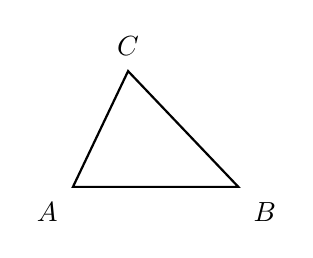
\begin{tikzpicture}[scale=0.7]
            \coordinate (A) at (0,0);
            \coordinate (B) at (3,0);
            \coordinate (C) at (1,2.1);
            \draw[thick] (A) -- (B) -- (C) -- cycle;
            \node[below left=2pt] at (A) {$A$};
            \node[below right=2pt] at (B) {$B$};
            \node[above=2pt] at (C) {$C$};
           
        \end{tikzpicture}
    \end{columns}
\end{frame}

% Example 1: Find the missing side (x)

% Question page
\begin{frame}{Example 1: Find the Missing Side / 例題1:求未知邊}
    \begin{tcolorbox}[colback=lightgray,colframe=primary,title=Question]
        In $\triangle ABC$, $B=25^\circ$, $c=15$, $a=7$. Find $b$.
    \end{tcolorbox}
    \vspace{0.5em}
    \begin{center}
    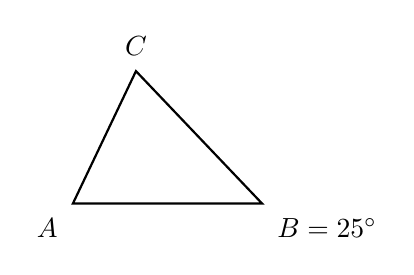
\begin{tikzpicture}[scale=0.8]
        \coordinate (A) at (0,0);
        \coordinate (B) at (3,0);
        \coordinate (C) at (1,2.1);
        \draw[thick] (A) -- (B) -- (C) -- cycle;
        \node[below left=2pt] at (A) {$A$};
        \node[below right=2pt] at (B) {$B=25^\circ$};
        \node[above=2pt] at (C) {$C$};
    \end{tikzpicture}
    \end{center}
\end{frame}

% Answer page
\begin{frame}{Example 1: Solution / 解答}
    \footnotesize
    \[
        b^2 = a^2 + c^2 - 2ac\cos B
    \]
    \[
        b^2 = 7^2 + 15^2 - 2 \times 7 \times 15 \cos 25^\circ
    \]
    \[
        b^2 = 49 + 225 - 210 \times 0.9063
    \]
    \[
        b^2 = 274 - 190.32 = 83.68
    \]
    \[
        b = \sqrt{83.68} \approx 9.15
    \]
\end{frame}

% Example 2: Find the missing side (x)

% Question page
\begin{frame}{Example 2: Find the Missing Side / 例題2:求未知邊}
    \begin{tcolorbox}[colback=lightgray,colframe=primary,title=Question]
        In $\triangle ABC$, $B=105^\circ$, $a=17$, $c=14$. Find $b$.
    \end{tcolorbox}
    \vspace{0.5em}
    \begin{center}
    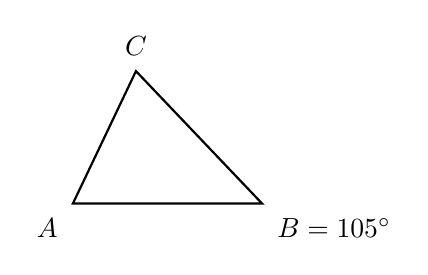
\begin{tikzpicture}[scale=0.8]
        \coordinate (A) at (0,0);
        \coordinate (B) at (3,0);
        \coordinate (C) at (1,2.1);
        \draw[thick] (A) -- (B) -- (C) -- cycle;
        \node[below left=2pt] at (A) {$A$};
        \node[below right=2pt] at (B) {$B=105^\circ$};
        \node[above=2pt] at (C) {$C$};
    \end{tikzpicture}
    \end{center}
\end{frame}

% Answer page
\begin{frame}{Example 2: Solution / 解答}
    \footnotesize
    \[
        b^2 = a^2 + c^2 - 2ac\cos B
    \]
    \[
        b^2 = 17^2 + 14^2 - 2 \times 17 \times 14 \cos 105^\circ
    \]
    \[
        b^2 = 289 + 196 - 476 \times (-0.2588)
    \]
    \[
        b^2 = 485 + 123.20 = 608.20
    \]
    \[
        b = \sqrt{608.20} \approx 24.66
    \]
\end{frame}

% II) Finding Angles with the Cosine Law

% Question page
\begin{frame}{II) Finding Angles with Cosine Law / 用餘弦定理求角}
    \begin{tcolorbox}[colback=lightgray,colframe=primary,title=Question]
        In $\triangle ABC$, $a=9$, $b=8$, $c=14$. Find $\theta$ (angle opposite $c$).
    \end{tcolorbox}
    \vspace{0.5em}
    \begin{center}
    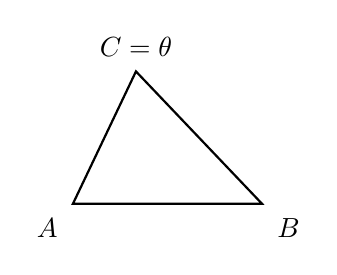
\begin{tikzpicture}[scale=0.8]
        \coordinate (A) at (0,0);
        \coordinate (B) at (3,0);
        \coordinate (C) at (1,2.1);
        \draw[thick] (A) -- (B) -- (C) -- cycle;
        \node[below left=2pt] at (A) {$A$};
        \node[below right=2pt] at (B) {$B$};
        \node[above=2pt] at (C) {$C=\theta$};
    \end{tikzpicture}
    \end{center}
\end{frame}

% Answer page
\begin{frame}{II) Solution / 解答}
    \footnotesize
    \[
        \cos \theta = \frac{a^2 + b^2 - c^2}{2ab}
    \]
    \[
        \cos \theta = \frac{9^2 + 8^2 - 14^2}{2 \times 9 \times 8} = \frac{81+64-196}{144} = \frac{-51}{144} \approx -0.3542
    \]
    \[
        \theta = \cos^{-1}(-0.3542) \approx 110.74^\circ
    \]
\end{frame}

% Practice: Find the missing angle

% Question page
\begin{frame}{Practice: Find the Missing Angle / 練習:求未知角}
    \begin{tcolorbox}[colback=lightgray,colframe=accent,title=Practice]
        In $\triangle ABC$, $a=12$, $b=15$, $c=8$. Find $C$.
    \end{tcolorbox}
    \vspace{0.5em}
    \begin{center}
    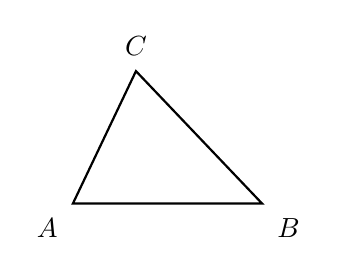
\begin{tikzpicture}[scale=0.8]
        \coordinate (A) at (0,0);
        \coordinate (B) at (3,0);
        \coordinate (C) at (1,2.1);
        \draw[thick] (A) -- (B) -- (C) -- cycle;
        \node[below left=2pt] at (A) {$A$};
        \node[below right=2pt] at (B) {$B$};
        \node[above=2pt] at (C) {$C$};
    \end{tikzpicture}
    \end{center}
\end{frame}

% Answer page
\begin{frame}{Practice: Solution / 解答}
    \footnotesize
    \[
        \cos C = \frac{a^2 + b^2 - c^2}{2ab}
    \]
    \[
        \cos C = \frac{12^2 + 15^2 - 8^2}{2 \times 12 \times 15}
    \]
    \[
        \cos C = \frac{144 + 225 - 64}{360} = \frac{305}{360} \approx 0.8472
    \]
    \[
        C = \cos^{-1}(0.8472) \approx 32.06^\circ
    \]
\end{frame}

% Example: Find the missing side with Cosine Law

% Question page
\begin{frame}{Example: Find the Missing Side / 例題:餘弦定理求邊}
    \begin{tcolorbox}[colback=lightgray,colframe=primary,title=Question]
        In $\triangle ABC$, $a=8$, $b=5$, $C=30^\circ$. Find $c$.
    \end{tcolorbox}
    \vspace{0.5em}
    \begin{center}
    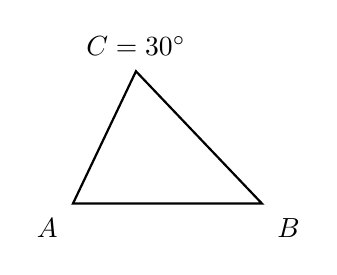
\begin{tikzpicture}[scale=0.8]
        \coordinate (A) at (0,0);
        \coordinate (B) at (3,0);
        \coordinate (C) at (1,2.1);
        \draw[thick] (A) -- (B) -- (C) -- cycle;
        \node[below left=2pt] at (A) {$A$};
        \node[below right=2pt] at (B) {$B$};
        \node[above=2pt] at (C) {$C=30^\circ$};
    \end{tikzpicture}
    \end{center}
\end{frame}

% Answer page
\begin{frame}{Example: Solution / 解答}
    \footnotesize
    \[
        c^2 = a^2 + b^2 - 2ab\cos C
    \]
    \[
        c^2 = 8^2 + 5^2 - 2 \times 8 \times 5 \cos 30^\circ
    \]
    \[
        c^2 = 64 + 25 - 80 \times 0.8660
    \]
    \[
        c^2 = 89 - 69.28 = 19.72
    \]
    \[
        c = \sqrt{19.72} \approx 4.44
    \]
\end{frame}

% Practice: Find the area of the triangle

% Question page
\begin{frame}{Practice: Find the Area / 練習:求三角形面積}
    \begin{tcolorbox}[colback=lightgray,colframe=accent,title=Practice]
        In $\triangle ABC$, $a=12$ cm, $b=27$ cm, $c=35$ cm. Find the area of the triangle.
    \end{tcolorbox}
    \vspace{0.5em}
    \begin{center}
    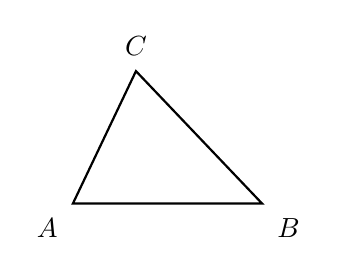
\begin{tikzpicture}[scale=0.8]
        \coordinate (A) at (0,0);
        \coordinate (B) at (3,0);
        \coordinate (C) at (1,2.1);
        \draw[thick] (A) -- (B) -- (C) -- cycle;
        \node[below left=2pt] at (A) {$A$};
        \node[below right=2pt] at (B) {$B$};
        \node[above=2pt] at (C) {$C$};
    \end{tikzpicture}
    \end{center}
\end{frame}

% Answer page
\begin{frame}{Practice: Solution / 解答}
    \footnotesize
    \textbf{Use Heron's formula or $Area = \frac{1}{2}ab\sin C$ after finding an angle.}
    \[
        s = \frac{12+27+35}{2} = 37
    \]
    \[
        Area = \sqrt{37(37-12)(37-27)(37-35)} = \sqrt{37 \times 25 \times 10 \times 2} \approx 136.01
    \]
    \text{(units$^2$)}
\end{frame}

% Proof for the Cosine Law
\begin{frame}{Proof for the Cosine Law / 餘弦定理證明}
    \begin{tcolorbox}[colback=lightgray,colframe=primary,title=Proof Sketch]
        \footnotesize
        \begin{columns}
            \column{0.5\textwidth}
            \begin{align*}
                &\text{Let $h$ be the height from $C$ to $AB$} \\
                &b^2 = h^2 + (x)^2 \\
                &c^2 = h^2 + (a-x)^2 \\
                &\text{Expand:} \\
                &c^2 = h^2 + a^2 - 2ax + x^2 \\
                &\text{Substitute $b^2 = h^2 + x^2$:} \\
                &c^2 = b^2 + a^2 - 2ax \\
                &\text{But $x = b\cos A$} \\
                &c^2 = a^2 + b^2 - 2ab\cos A
            \end{align*}
            \column{0.5\textwidth}
            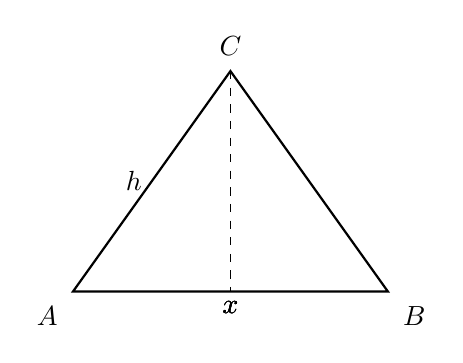
\begin{tikzpicture}[scale=1]
                \coordinate (A) at (0,0);
                \coordinate (B) at (4,0);
                \coordinate (C) at (2,2.8);
                \draw[thick] (A) -- (B) -- (C) -- cycle;
                \draw[dashed] (C) -- (2,0);
                \node[below left=2pt] at (A) {$A$};
                \node[below right=2pt] at (B) {$B$};
                \node[above=2pt] at (C) {$C$};
                \node[below] at (2,0) {$x$};
                \node[left] at (1,1.4) {$h$};
                \node[below] at (2,0) {$x$};
                \node[below] at (2,0) {$x$};
                \node[below] at (2,0) {$x$};
            \end{tikzpicture}
        \end{columns}
    \end{tcolorbox}
\end{frame}

\end{document} 